\documentclass[border=2mm]{standalone}
\usepackage{color}
\usepackage{tikz}

\usetikzlibrary{shapes,arrows,arrows.meta,fit,positioning}

\newcommand{\defaultside}{4cm}

\tikzset{
    auto, node distance = 2cm,
    stage/.style = { draw, thick, rectangle, align=center,
        text width = \defaultside, 
        font=\bfseries,
        rounded corners=2mm, 
        minimum width = \defaultside
    },
    note/.style = { draw, very thin, rectangle, dashed, align=center,
        node distance = 0.5cm,
        text width = \defaultside - 1cm, 
        font=\footnotesize,
        minimum width = \defaultside - 1cm
    },
    arrow/.style = { -latex, very thick },
    arrow_text/.style = { align=center,
        pos = 0.5,
        text width = 3cm, 
        font = \scriptsize
    }
}

\begin{document}
    \begin{tikzpicture}
        \node[stage] (0) at (0,0) {Zona seleccionada \\ 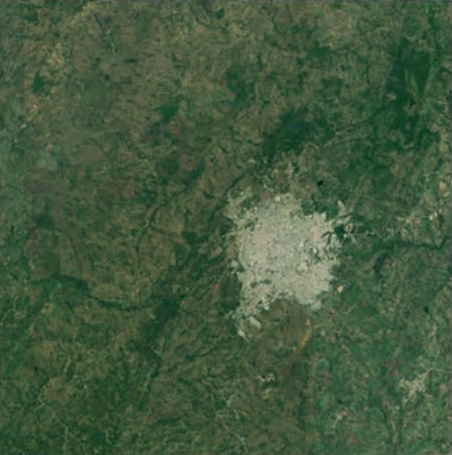
\includegraphics[width=\defaultside, height=\defaultside]{example_without_crops_1}};
        %\node[scale=1.5] (A) [below = 2mm of 0] {(a)};
        
        \node[stage] (1) [right = 5mm of 0] {Composición \\ 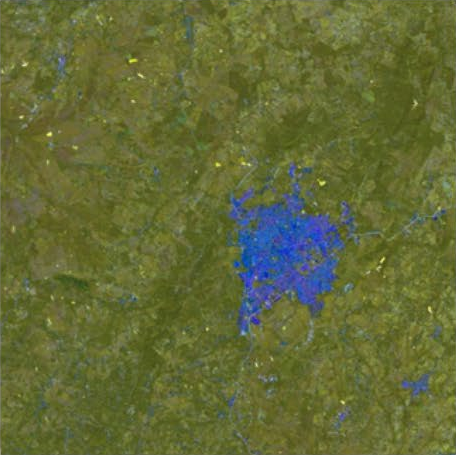
\includegraphics[width=\defaultside, height=\defaultside]{example_without_crops_2}};
        %\node[scale=1.5] (B) [below = 2mm of 1] {(b)};
        
        \node[stage] (2) [right = 5mm of 1] {Predicción \\ 
\includegraphics[width=\defaultside, height=\defaultside]{example_without_crops_3}};
        %\node[scale=1.5] (C) [below = 2mm of 2] {(c)};
        
        %\draw[arrow] (0) --  (1);
        %\draw[arrow] (1) --  (2);
    \end{tikzpicture}
\end{document}
